\documentclass[11pt,preprint, authoryear]{elsarticle}

\usepackage{lmodern}
%%%% My spacing
\usepackage{setspace}
\setstretch{1.2}
\DeclareMathSizes{12}{14}{10}{10}

% Wrap around which gives all figures included the [H] command, or places it "here". This can be tedious to code in Rmarkdown.
\usepackage{float}
\let\origfigure\figure
\let\endorigfigure\endfigure
\renewenvironment{figure}[1][2] {
    \expandafter\origfigure\expandafter[H]
} {
    \endorigfigure
}

\let\origtable\table
\let\endorigtable\endtable
\renewenvironment{table}[1][2] {
    \expandafter\origtable\expandafter[H]
} {
    \endorigtable
}


\usepackage{ifxetex,ifluatex}
\usepackage{fixltx2e} % provides \textsubscript
\ifnum 0\ifxetex 1\fi\ifluatex 1\fi=0 % if pdftex
  \usepackage[T1]{fontenc}
  \usepackage[utf8]{inputenc}
\else % if luatex or xelatex
  \ifxetex
    \usepackage{mathspec}
    \usepackage{xltxtra,xunicode}
  \else
    \usepackage{fontspec}
  \fi
  \defaultfontfeatures{Mapping=tex-text,Scale=MatchLowercase}
  \newcommand{\euro}{€}
\fi

\usepackage{amssymb, amsmath, amsthm, amsfonts}

\def\bibsection{\section*{References}} %%% Make "References" appear before bibliography


\usepackage[round]{natbib}

\usepackage{longtable}
\usepackage[margin=2.3cm,bottom=2cm,top=2.5cm, includefoot]{geometry}
\usepackage{fancyhdr}
\usepackage[bottom, hang, flushmargin]{footmisc}
\usepackage{graphicx}
\numberwithin{equation}{section}
\numberwithin{figure}{section}
\numberwithin{table}{section}
\setlength{\parindent}{0cm}
\setlength{\parskip}{1.3ex plus 0.5ex minus 0.3ex}
\usepackage{textcomp}
\renewcommand{\headrulewidth}{0.2pt}
\renewcommand{\footrulewidth}{0.3pt}

\usepackage{array}
\newcolumntype{x}[1]{>{\centering\arraybackslash\hspace{0pt}}p{#1}}

%%%%  Remove the "preprint submitted to" part. Don't worry about this either, it just looks better without it:
\makeatletter
\def\ps@pprintTitle{%
  \let\@oddhead\@empty
  \let\@evenhead\@empty
  \let\@oddfoot\@empty
  \let\@evenfoot\@oddfoot
}
\makeatother

 \def\tightlist{} % This allows for subbullets!

\usepackage{hyperref}
\hypersetup{breaklinks=true,
            bookmarks=true,
            colorlinks=true,
            citecolor=blue,
            urlcolor=blue,
            linkcolor=blue,
            pdfborder={0 0 0}}


% The following packages allow huxtable to work:
\usepackage{siunitx}
\usepackage{multirow}
\usepackage{hhline}
\usepackage{calc}
\usepackage{tabularx}
\usepackage{booktabs}
\usepackage{caption}


\newenvironment{columns}[1][]{}{}

\newenvironment{column}[1]{\begin{minipage}{#1}\ignorespaces}{%
\end{minipage}
\ifhmode\unskip\fi
\aftergroup\useignorespacesandallpars}

\def\useignorespacesandallpars#1\ignorespaces\fi{%
#1\fi\ignorespacesandallpars}

\makeatletter
\def\ignorespacesandallpars{%
  \@ifnextchar\par
    {\expandafter\ignorespacesandallpars\@gobble}%
    {}%
}
\makeatother

\newenvironment{CSLReferences}[2]{%
}

\urlstyle{same}  % don't use monospace font for urls
\setlength{\parindent}{0pt}
\setlength{\parskip}{6pt plus 2pt minus 1pt}
\setlength{\emergencystretch}{3em}  % prevent overfull lines
\setcounter{secnumdepth}{5}

%%% Use protect on footnotes to avoid problems with footnotes in titles
\let\rmarkdownfootnote\footnote%
\def\footnote{\protect\rmarkdownfootnote}
\IfFileExists{upquote.sty}{\usepackage{upquote}}{}

%%% Include extra packages specified by user

%%% Hard setting column skips for reports - this ensures greater consistency and control over the length settings in the document.
%% page layout
%% paragraphs
\setlength{\baselineskip}{12pt plus 0pt minus 0pt}
\setlength{\parskip}{12pt plus 0pt minus 0pt}
\setlength{\parindent}{0pt plus 0pt minus 0pt}
%% floats
\setlength{\floatsep}{12pt plus 0 pt minus 0pt}
\setlength{\textfloatsep}{20pt plus 0pt minus 0pt}
\setlength{\intextsep}{14pt plus 0pt minus 0pt}
\setlength{\dbltextfloatsep}{20pt plus 0pt minus 0pt}
\setlength{\dblfloatsep}{14pt plus 0pt minus 0pt}
%% maths
\setlength{\abovedisplayskip}{12pt plus 0pt minus 0pt}
\setlength{\belowdisplayskip}{12pt plus 0pt minus 0pt}
%% lists
\setlength{\topsep}{10pt plus 0pt minus 0pt}
\setlength{\partopsep}{3pt plus 0pt minus 0pt}
\setlength{\itemsep}{5pt plus 0pt minus 0pt}
\setlength{\labelsep}{8mm plus 0mm minus 0mm}
\setlength{\parsep}{\the\parskip}
\setlength{\listparindent}{\the\parindent}
%% verbatim
\setlength{\fboxsep}{5pt plus 0pt minus 0pt}



\begin{document}



\begin{frontmatter}  %

\title{Using SQL Queries}

% Set to FALSE if wanting to remove title (for submission)




\author[Add1]{Anna Mayer}
\ead{28776534@sun.ac.za}





\address[Add1]{Stellenbosch University}


\begin{abstract}
\small{
This report analyses price changes due to inflation in South Africa and
proposes a new index - the braaibrodje index.
}
\end{abstract}

\vspace{1cm}


\begin{keyword}
\footnotesize{
CPI \sep Braai \sep Inflation \\
\vspace{0.3cm}
}
\end{keyword}



\vspace{0.5cm}

\end{frontmatter}

\setcounter{footnote}{0}



%________________________
% Header and Footers
%%%%%%%%%%%%%%%%%%%%%%%%%%%%%%%%%
\pagestyle{fancy}
\chead{}
\rhead{}
\lfoot{}
\rfoot{\footnotesize Page \thepage}
\lhead{}
%\rfoot{\footnotesize Page \thepage } % "e.g. Page 2"
\cfoot{}

%\setlength\headheight{30pt}
%%%%%%%%%%%%%%%%%%%%%%%%%%%%%%%%%
%________________________

\headsep 35pt % So that header does not go over title




\hypertarget{introduction}{%
\section{\texorpdfstring{Introduction
\label{Introduction}}{Introduction }}\label{introduction}}

Using a novel approach with the braaibrodjie index, this report aims to
visualize the impact of inflation. Two data sets are used for the
analysis and the results for the indices are compared. Further, general
summary statistics and price development in general over time are part
of the report.

\hypertarget{data}{%
\section{Data}\label{data}}

Two data sets were provided. One on retailer prices. The other one
contains data from StatsSA. Note that the StatsSA data set was adjusted
such that the two data sets cover the same periods.

\hypertarget{analysis}{%
\section{Analysis}\label{analysis}}

\hypertarget{a-braaibrodje-index}{%
\subsection{A Braaibrodje index}\label{a-braaibrodje-index}}

Given the two data sets provided, two different braaibrodjies indices
are calculated and plotted separately for the two different data sets.\\

\begin{figure}[H]

{\centering \includegraphics{Question5_files/figure-latex/Figure1-1} 

}

\caption{Braaibrodjie Index Stats SA Retailer \label{Figure1}}\label{fig:Figure1}
\end{figure}

Already in this graph, we can see, that the prices have been increasing
significantly over the pat years. In a next step, we will have a look at
the index over time from the other data set.

\begin{figure}[H]

{\centering 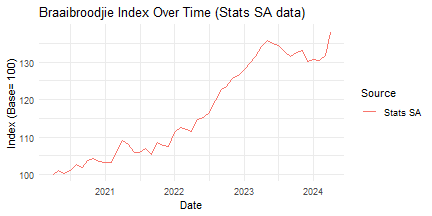
\includegraphics{Question5_files/figure-latex/Figure2-1} 

}

\caption{Braaibrodjie Index Stats SA \label{Figure2}}\label{fig:Figure2}
\end{figure}

As one can clearly see in both graphs, prices have increased int he past
three years. As the braaibrodjie index from the Retailer data shows
clearly a larger increase in prices, it might be the case that the data
from StatsSA is underestimating the true inflation. Nevertheless, no
quantities were given to which the prices relate in the StatsSA data,
which leaves us with speculation whether we can assume that the prices
relate to the same quantities.

To have a closer look into general summary statistics of the data set,
please continue with the next section. \#\# B - Summary Statistics and
comparison of the data First, this report compares mean prices of the
different ingredients for Braaibrodjie to check whether the data sets
have similar price observations.

\begin{figure}[H]

{\centering \includegraphics{Question5_files/figure-latex/Figure3-1} 

}

\caption{Summary Statistics \label{Figure3}}\label{fig:Figure3}
\end{figure}

Again, one can see that the Stats SA and the Retailer data sets use
different prices. One wonders whether this is due to different
quantities, they are referring to or whether there are other reasons for
the difference in prices.

Finally, this report looks at the price development of tomatoes over the
past three years in the two different data sets.

\begin{figure}[H]

{\centering 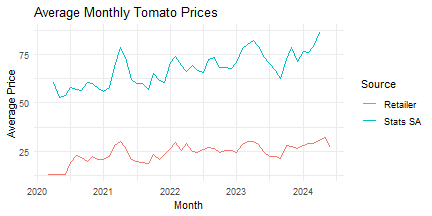
\includegraphics{Question5_files/figure-latex/Figure4-1} 

}

\caption{Tomato Prices over Time \label{Figure4}}\label{fig:Figure4}
\end{figure}

Tomato prices have been increasing in both data sets which is also in
line with the increasing braaibrodjies index in both data sets.

Based on other estimates, annual consumer price inflation was 5,2\% in
April 2024, down from the 5,3\% in March 2024.The consumer price index
increased by 0,3\% in April 2024.

\hypertarget{conclusion}{%
\section{Conclusion}\label{conclusion}}

The braaibrodjie index provides a hands on understandable, especially
for the South African context, index for inflation. It is similar to the
big mac index that has been used for several years now. However, for the
South Africa, a braaibrodjie index seems more fitting. In the graphs
provided, one could clearly see the inflation patterns and price
increases which were visible in both data sets based on the novel index.

\bibliography{Tex/ref}





\end{document}
